\documentclass[12pt,a4paper,notitlepage]{article}

\usepackage[utf8]{inputenc}

\usepackage[francais]{babel}\usepackage[T1]{fontenc}
\usepackage[cyr]{aeguill}
\usepackage{lmodern}

\usepackage{amssymb}
\usepackage[table]{xcolor}
\definecolor{gris}{gray}{0.75}
\definecolor{bleup}{HTML}{258EE9}


%\renewcommand*\familydefault{\ttdefault} %% Only if the base font of the document is to be typewriter style
%\renewcommand{\rmdefault}{ptm}


\usepackage[
   pdfauthor={Ludovic Terrier & Arnaud Goulut},
   pdftitle={RE12 - TP1},
   ]{hyperref}
   
   
\usepackage[pdftex]{graphicx}

%\usepackage{titlesec}
%\titleformat{\section}[frame] {\normalfont} {\filright
%\footnotesize
%\enspace\textbf{\thesection}\enspace} {8pt} {\Large\bfseries\filcenter}

%% Je contrôle la taille de ma zone imprimée...
\usepackage{anysize}
%% ...en définissants les marges {gauche}{droite}{haute}{basse}
\marginsize{25mm}{15mm}{10mm}{15mm}

\begin{document}

\title{La configuration réseau sous Linux}
\author{Ludovic Terrier et Arnaud Goulut}
\date{Mars 2010}
\maketitle


%\tableofcontents

\thispagestyle{empty}
\newpage

%%%%%%%%%%%%%%%%%%%%%%%%%%%%%%%%%%%  1ère page 


%%%%%%%%%%%%%%%%%%%%%%%%%%%%%%%%%%% 1ère partie
\section{Partie 1}

\subsection{Question 1}
\begin{figure}[!h]
\begin{center}
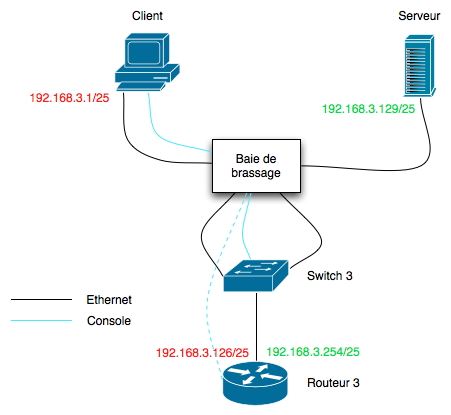
\includegraphics[height=11cm]{Diag.png}
\caption{Présentation du réseau configuré au cours du TP.}
\label{fig:do}
\end{center}
\end{figure}
\subsection{Question 2}


\begin{center}
\rowcolors{1}{gris}{}
\begin{tabular}{|c|c|}
  \hline
 \multicolumn{2}{|c|}{\cellcolor{bleup}Réseau du client} \\
  \hline
  NetID & 192.168.3.0 \\
  Masque & /25  \\
  Plage d'adresse & 192.168.3.0 - 192.168.3.127\\
  1\up{ère} adresse machine & 192.168.3.1\\
  Dernière adresse machine & 192.168.2.126\\
  Nombre de machines potentiel & 126\\
  Broadcast & 192.168.3.127\\
  \hline
\end{tabular}
\end{center}

\begin{center}
\rowcolors{1}{gris}{}
\begin{tabular}{|c|c|}
  \hline
  \rowcolor{orangec} \multicolumn{2}{|c|}{\cellcolor{bleup}Réseau du seveur} \\
  \hline
  NetID & 192.168.3.128 \\
  Masque & /25  \\
  Plage d'adresse & 192.168.3.128 - 192.168.3.255\\
  1\up{ère} adresse machine & 192.168.3.129\\
  Dernière adresse machine& 192.168.3.254\\
  Nombre de machines potentiel & 126\\
  Broadcast & 192.168.3.255\\
  \hline
\end{tabular}
\end{center}

\begin{center}
\rowcolors{1}{gris}{}
\begin{tabular}{|c|c|}
  \hline
  \rowcolor{orangec} \multicolumn{2}{|c|}{\cellcolor{bleup}Réseau de transport} \\
  \hline
  NetID & 172.16.3.0 \\
  Masque & /30  \\
  Plage d'adresse & 172.16.3.0 - 172.16.3.3\\
  1\up{ère} adresse machine & 172.16.3.1\\
  Dernière adresse machine&  172.16.3.2\\
  Nombre de machines potentiel & 2\\
  Broadcast & 172.16.3.3\\
  \hline
\end{tabular}
\end{center}

\paragraph{}Dans les réseaux du serveur et du client on utilise un seul réseau (192.168.3.0) de classe C. Cependant pour en faire deux réseaux distincts on le scinde à l'aide du masque : $\mathtt{/25}$. Ceci signifie que les 25 premiers bits de chaque adresse IP utilisée sur le réseau correspondra au NetID et les 7 derniers au HostID. On obtient donc 2 sous-réseaux ayant pour adresse respective : 192.168.3.0 et 192.168.3.128.

\paragraph{}Dans le cas du réseau de transport, nous avons un réseau 172.16.3.0, qui contiendra seulement deux machines. C'est pourquoi on peut se permettre d'utiliser un masque $\mathtt{/30}$ qui, appliqué à notre réseau de départ donne 4 adresses : 
\begin{itemize}
\item deux adresses à utiliser pour des hosts,
\item une pour le broadcast,
\item une pour le NetID.
\end{itemize}


\subsection{Question 3}

Pour l'administration de matériel réseaux on préfère utiliser un port console dédié. Ceci afin d'assurer l'accès à l'équipement en cas d'une mauvaise manipulation, qui le rendrait inaccessible via ses interfaces réseaux (Ethernet dans le cadre des TPs) ou dans le cas d'une congestion du réseau.

Cette interface est un port série (avec connectique RJ45 / DB9) 


\section{Partie 2}
\subsection{Configuration du switch}

Le switch peut-être logiquement séparé en deux grâce aux Virtual Local Area Networks (VLANs). Une différenciation des deux VLANs peut se faire par ports, ce qui se voit dans le fichier de configuration des switchs, seul le port \textit{FastEthernet0/2} est attribué à un VLAN :

\begin{center}
\fbox{
	\begin{minipage}{8cm}
	\hspace{2cm}\vdots\\
	interface FastEthernet0/2\\                        
	 switchport access vlan 2 
	 
	 
	 \hspace{2cm}\vdots
	 \end{minipage}
}
 \end{center}
 
Ce qui peut vouloir dire que l'ensemble des autres ports sont dans le même VLAN par défaut.

\subsection{Configuration du routeur}
\paragraph{}Le switch de notre réseau étant relié au routeur par un seul médium et que celui-ci transporte les flux de deux sous-réseaux, il faut que l'interface routeur soit elle-même séparée en deux interfaces logiques. Ce qui semble fait au regard du fichier de configuration du routeur :


\begin{center}
\fbox{
	\begin{minipage}{8cm}
	\hspace{2cm}\vdots\\
	interface FastEthernet0/0\textbf{.1}\\                           
	 encapsulation dot1Q 1 native\\                             
	 ip address 192.168.3.126 255.255.255.128\\                                         
	! \\
	interface FastEthernet0/0\textbf{.2}          \\                 
	 encapsulation dot1Q 2               \\
	 ip address 192.168.3.254 255.255.255.128  
	 
	 
	 \hspace{2cm}\vdots
	 \end{minipage}
}
 \end{center}



L'interface \textit{FastEthernet0/0} du routeur à laquelle est connectée le switch est partagée en deux : 
\begin{itemize}
\item \textbf{.1} pour le réseau 192.168.3.0 (l'interface ayant l'adresse 192.168.3.126)
\item \textbf{.2 }pour le réseau 192.168.3.128 (l'interface ayant l'adresse 192.168.3.254)
\end{itemize}


\section{Partie 3}
\subsection{Question 1}
Pour communiquer sur un réseau, une machine à besoin au minimum, d'une adresse IP, d'un masque et d'une passerelle par défaut. Ce sont donc ces informations que l'on peut stocker dans le fichier $\mathtt{/etc/sysconfig/network}$

\subsection{Question 2}
\paragraph{}En lisant le fichier $\mathtt{/etc/modprobe.conf}$ on peut lire la ligne :

\begin{center}
\fbox{
	\begin{minipage}{8cm}
	\hspace{2cm}\vdots\\
	alias eth1 e1000e
	 
	 
	 \hspace{2cm}\vdots
	 \end{minipage}
}
 \end{center}

Ce qui signifie que l'alias \textit{eth1} est créé vers le pilote (\textit{e1000e}) de la carte réseau. Si l'on effectue la commande \textit{ifconfig} dans un Terminal on pourra observer \textit{eth1} et pas \textit{e1000e}.

\subsection{Question 3}

Les paramètres que l'on peut attribuer à une interface réseau avec la commande \textit{ifconfig} sont l'adresse IP et le masque de sous réseau.

ifconfig \textless interface\textgreater\  \textless adresse\_IP\textgreater\ netmask \textless masque\textgreater

Pour le Client :
ifconfig eth1 192.168.3.1 netmask 255.255.255.128


Pour le Serveur :
ifconfig eth1 192.168.3.129 netmask 255.255.255.128 


\subsection{Question 4}

Ces mêmes informations peuvent-être conservées de manière pérenne dans le dossier :

$\mathtt{/etc/sysconfig/network-scripts/ifcfg-\textless interface\textgreater}$ 

ou dans notre cas $\mathtt{/etc/sysconfig/network-scripts/ifcfg-eth1}$ 
\end{document}
